\documentclass{article}
\usepackage{graphicx}

\begin{document}

1. simulation results from classroom data
\\\\\\\\\
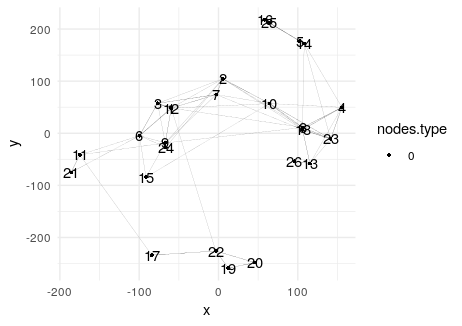
\includegraphics[scale=1]{classroom_t1.png}
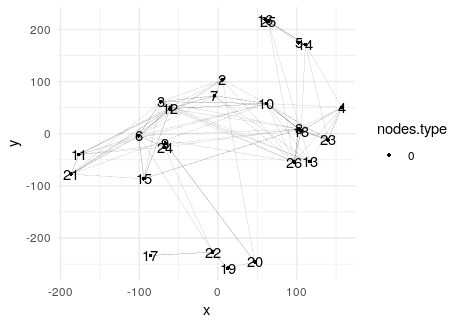
\includegraphics[scale=1]{classroom_t2.png}
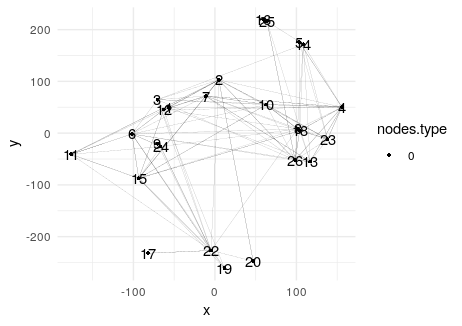
\includegraphics[scale=1]{classroom_t3.png}
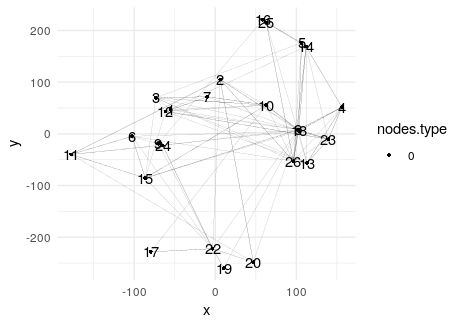
\includegraphics[scale=1]{classroom_t4.png}
\\
2. Poisson regression type for count data\\
From Dan's paper about weighted edges,
$$
\log (\mu) = \eta,$$

$$
y \sim Poisson(\mu)
$$
where $\eta$ is defined as before. \\
Derived likelihood function would be the product of each single link:
$$
-\mu + y \eta - \log(\Gamma(y+1))
$$

3. Partial set of links\\
For undirected network, we only need to consider link between node $i$ and $j$ where $i \leq j$. Similarly, when we are only interested in a subset of link types (e.g. when we are not interested in word-word link), we do not include other types of links in the likelihood.

\end{document}